\normaltrue \difficilefalse \tdifficilefalse
\correctionfalse
%\UPSTIidClasse{11} % 11 sup, 12 spé
%\newcommand{\UPSTIidClasse}{11}

\exer{ $\star$ \label{C2:03:prec:64}}
%% CCP MP 2007
\setcounter{question}{0}\UPSTIcompetence[2]{C2-03}
\index{Compétence C2-03}
\index{Schéma-blocs}
\index{Précision}

\ifcorrection
\else
\marginnote{\textbf{Pas de corrigé pour cet exercice.}}
\fi


\ifprof
\else
On donne le système suivant dont la la FTBF est donnée par 
$G(p)=\dfrac{\Theta_S(p)}{\Theta_C(p)}=\dfrac{3,24}{p^2+3,24 p+3,24}$. Le retard du système est de \SI{0,2}{s}.

L'asservissement est donné par le schéma-blocs suivant.

\begin{center}
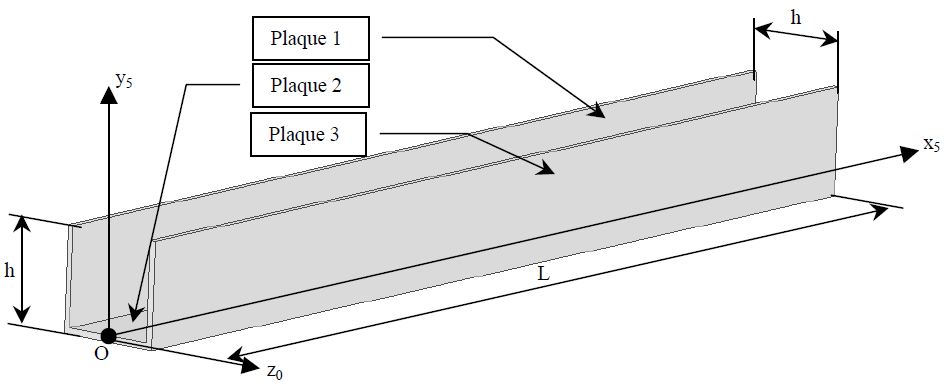
\includegraphics[width=.7\linewidth]{64_01}
\end{center}

\fi

 
\question{En considérant le retard nul, déterminer l'écart statique.}
\ifprof
\else 
\fi

\question{En considérant le retard nul, déterminer l'écart statique, déterminer l'expression de la boucle ouverte $H_{\text{BO}}(p)$.}
\ifprof
\else 
\fi
 
\question{Déterminer l'expression de $G_r(p)$, transmittance en boucle fermée du système avec retard de \SI{0,2}{s}.}
\ifprof
\else 
\fi
Le système est soumise à une rampe de \SI{0,1}{rad.s^{-1}}.
 
\question{Donner la valeur de l’erreur de traînage correspondant à cette entrée, en
négligeant le retard.}
\ifprof
\else 
\fi
 
\question{Donner la valeur de l'écart statique du système avec retard.}
\ifprof
\else 
\fi
 
\question{Donner la valeur de l'erreur de traînage du système avec retard.}
\ifprof
\else 
\fi

\ifprof
\else

\noindent\footnotesize
% \fbox{\parbox{.9\linewidth}{
% Éléments de corrigé : 
% \begin{enumerate}
  % \item $\varepsilon_{\text{con \%}} = \dfrac{1}{1+K_PK_m K_{\text{pom}} K_{\text{cap}} }$;
  % \item $K_P > 19$;
  % \item $\varepsilon_{\text{pert}} = \Delta Q_e \dfrac{K_f}{1+K_{\text{cap}}K_PK_mK_{\text{pom}}}$;
  % \item $K_P > 2,19$.
  % \item $K_P < 0,125$. Il est impossible de vérifier les trois conditions avec un correcteur proportionnel.
% \end{enumerate}}}
\normalsize

\begin{flushright}
\footnotesize{Corrigé  voir \ref{C2:03:prec:64}.}
\end{flushright}%
\fi